\section{方法比较与计算成本}
\label{sec:pm-comparison}

本节回答一个实际问题：同一个约束问题，四种方法到底哪里不同，比较代价时应该数什么。

\paragraph{各方法改变了什么}
四种方法都在做同一件事，把约束的信息换成原始变量子问题里的一项。它们的差别可以按三个方面读出来：给目标加了什么，乘子怎样更新，原始变量怎样求解。

\begin{BookInlineTable}
  \centering
  \small
  \begin{tabular}{@{}llll@{}}
    \toprule
    方法 & 目标的改动 & 乘子 & 原始变量\\
    \midrule
    二次罚 & 加平方罚 & 无（$\rho h$仅作估计） & 逐轮全部求解\\
    一次罚 & 加一次罚 & 无（门槛内隐含） & 非光滑子问题\\
    对偶上升 & 加线性价格 & 显式步 & 可分块，全部求解\\
    ALM & 价格加平方罚 & 隐式步，步长$\rho$ & 联合求解\\
    ADMM & 价格加平方罚 & 步长$\rho$ & 两块各更新一次\\
    \bottomrule
  \end{tabular}
  \caption{各方法的结构对照。}
  \label{tab:pm-structure}
\end{BookInlineTable}

\paragraph{相同精度下的代价}
比较时要固定口径。各方法的罚目标函数不同，比较目标值没有意义；ADMM的一轮和ALM的一轮完成的工作也不同，比较轮数同样没有意义。合理的办法是固定同一个问题，要求达到相同的原始精度，再分别统计外层轮数、内层计算和通信。

下面用二元例，都从原点出发，要求$\lvert h(\bm{x})\rvert\leq10^{-3}$。内层的梯度法取步长$1/L$，容差为$10^{-6}$，这样内层误差不干扰外层。ADMM的两个子问题都是一元二次函数的最小化，取闭式解。

\begin{BookInlineTable}
  \centering
  \small
  \begin{tabular}{@{}lrrrr@{}}
    \toprule
    方法 & 外层轮数 & 内层梯度步 & 矩阵分解 & 最大条件数\\
    \midrule
    二次罚（$\rho$乘$10$） & $5$ & $123443$ & $5$ & $15001$\\
    对偶上升（$\alpha=0.6$） & $7$ & $162$ & $0$ & $3$\\
    ALM（$\rho=1.5$） & $8$ & $230$ & $1$ & $3.1$\\
    ADMM（$\rho=1.5$） & $11$ & 闭式 & $0$ & 无\\
    \bottomrule
  \end{tabular}
  \caption{二元例中达到$\lvert h\rvert\leq10^{-3}$的代价。“矩阵分解”指改用直接法解内层时需要的分解次数。这些数字只对这个例子有效。}
  \label{tab:pm-cost}
\end{BookInlineTable}

表~\ref{tab:pm-cost}和图~\ref{fig:pm-compare}说明了几件事。二次罚外层轮数最少，内层步数却多出几个数量级，几乎全部花在最后两轮的病态问题上。ALM比二次罚多几轮，却始终在解同一个良态问题。

对偶上升在这里表现很好，因为$f$是强凸的，内层矩阵的条件数只有$3$，步长也事先选好了。如果把目标改成线性的，或者步长取到$1.5$，它就失效了，表中的数字不能外推。ADMM在这里每个子问题都是一元的，所以一轮很便宜，但一轮要交换一次信息。在通信比本地计算贵得多的环境中，轮数才是主要成本。

\begin{BookInlineFigure}
  \centering
  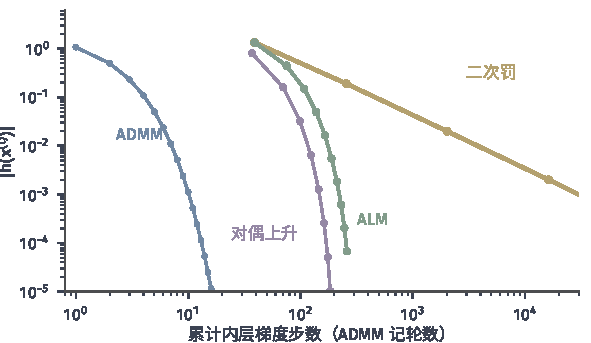
\includegraphics[width=100mm]{figures/05-optimization/06-constrained-optimization/matplotlib/pm-compare/figure.pdf}
  \caption{二元例上约束残差随累计计算量的下降，双对数坐标。黄线是二次罚，紫线是对偶上升，绿线是ALM，横轴是累计的梯度步数（内层容差$10^{-6}$）；蓝线是ADMM，横轴是轮数，两者的单位不同，只宜比较曲线的走势。}
  \label{fig:pm-compare}
\end{BookInlineFigure}

\paragraph{比较时容易出错的地方}
第一，不同方法的罚目标值不可比。$Q_\rho$、$E_\rho$、$\mathcal{L}_\rho$的数值里都混有罚项，要比较的是原目标和约束违规，或者驻定残差。

第二，只比较一次内层更新的速度会误导。一次梯度步的时间四种方法差不多，但需要多少步完全取决于子问题的条件数；对偶上升的内层便宜，可能需要更多外层轮数。

第三，精度要对等。一个方法返回约束残差$10^{-3}$的点，另一个返回$10^{-6}$的点，前者的目标值可能因为更不可行而显得更低。

第四，不同方法适用的问题不同，这个例子凸、光滑、约束线性。约束非线性时，对偶上升和ADMM的结论都要重新检查；目标非凸时，ALM的局部结论才是相关的。选择方法时应先看问题的结构：约束少而目标规模大时考虑ALM，目标和约束可分时考虑对偶分解或ADMM，只需要中等精度且子问题便宜时考虑ADMM，需要高精度时考虑ALM或者后面两章的方法。
